\begin{figure}[H]
    \centering

    \begin{subfigure}[t]{.45\textwidth}
        \centering
        \begingroup
  \sbox{\tempbox}{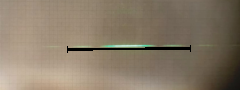
\includegraphics[width=\textwidth,page=1]{figuras/medidas/A1.pdf}}
  \begin{picture}(\wd\tempbox,\ht\tempbox)
    \put(0,0){\usebox{\tempbox}}
    \put(.48\wd\tempbox,.33\ht\tempbox){$2~\Delta y$}
  \end{picture}
\endgroup


        \caption{A1}
        \label{fig:A1}
    \end{subfigure}
    \qquad
    \begin{subfigure}[t]{.45\textwidth}
        \centering
        \begingroup
  \sbox{\tempbox}{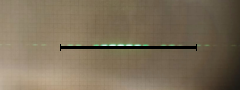
\includegraphics[width=\textwidth,page=1]{figuras/medidas/A2.pdf}}
  \begin{picture}(\wd\tempbox,\ht\tempbox)
    \put(0,0){\usebox{\tempbox}}
    \put(0,0){\includegraphics[width=\textwidth,page=2]{figuras/medidas/A2.pdf}}
    \put(.50\wd\tempbox,.35\ht\tempbox){$2~\Delta y$}
    \put(.485\wd\tempbox,.54\ht\tempbox){$6\Lambda$}
  \end{picture}
\endgroup


        \caption{A2}
        \label{fig:A2}
    \end{subfigure}
    \qquad
    \begin{subfigure}[t]{.45\textwidth}
        \centering
        \begingroup
  \sbox{\tempbox}{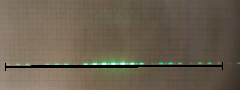
\includegraphics[width=\textwidth,page=1]{figuras/medidas/A3.pdf}}
  \begin{picture}(\wd\tempbox,\ht\tempbox)
    \put(0,0){\usebox{\tempbox}}
    \put(0,0){\includegraphics[width=\textwidth,page=2]{figuras/medidas/A3.pdf}}
    \put(.46\wd\tempbox,.15\ht\tempbox){$3~\Delta y$}
    \put(.44\wd\tempbox,.33\ht\tempbox){$2\delta y$}
  \end{picture}
\endgroup


        \caption{A3}
        \label{fig:A3}
    \end{subfigure}
    \qquad
    \begin{subfigure}[t]{.45\textwidth}
        \centering
        \begingroup
  \sbox{\tempbox}{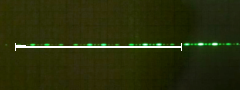
\includegraphics[width=\textwidth,page=1]{figuras/medidas/A4.pdf}}
  \begin{picture}(\wd\tempbox,\ht\tempbox)
    \put(0,0){\usebox{\tempbox}}
    \put(0,0){\includegraphics[width=\textwidth,page=2]{figuras/medidas/A4.pdf}}
    \put(.37\wd\tempbox,.35\ht\tempbox){\color{white}$1.5~\Delta y$}
    \put(.745\wd\tempbox,.56\ht\tempbox){\color{white}$2\delta y$}
  \end{picture}
\endgroup


        \caption{A4}
        \label{fig:A4}
    \end{subfigure}
    \qquad
    \begin{subfigure}[t]{.45\textwidth}
        \centering
        \begingroup
  \sbox{\tempbox}{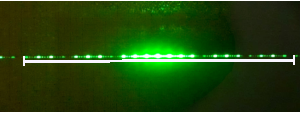
\includegraphics[width=\textwidth,page=1]{figuras/medidas/A5.pdf}}
  \begin{picture}(\wd\tempbox,\ht\tempbox)
    \put(0,0){\usebox{\tempbox}}
    \put(0,0){\includegraphics[width=\textwidth,page=2]{figuras/medidas/A5.pdf}}
    \put(.30\wd\tempbox,.33\ht\tempbox){\color{white}$3~\Delta y$}
    \put(.88\wd\tempbox,.54\ht\tempbox){\color{white}$2\delta y$}
  \end{picture}
\endgroup


        \caption{A5}
        \label{fig:A5}
    \end{subfigure}
    \qquad
    \begin{subfigure}[t]{.45\textwidth}
        \centering
        \begingroup
  \sbox{\tempbox}{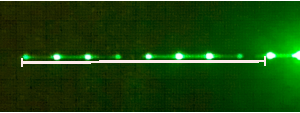
\includegraphics[width=\textwidth,page=1]{figuras/medidas/A6.pdf}}
  \begin{picture}(\wd\tempbox,\ht\tempbox)
    \put(0,0){\usebox{\tempbox}}
    \put(0,0){\includegraphics[width=\textwidth,page=2]{figuras/medidas/A6.pdf}}
    \put(.42\wd\tempbox,.32\ht\tempbox){\color{white}$1~\Delta y$}
    \put(.46\wd\tempbox,.56\ht\tempbox){\color{white}$2\delta y$}
  \end{picture}
\endgroup


        \caption{A6}
        \label{fig:A6}
    \end{subfigure}

    \caption{Fotos dos padrões de difração das fendas A}
    \label{fig:A}
\end{figure}